% ARPEGOS:  Automatized Roleplaying-game Profile Extensible Generator Ontology based System %
% Author : Alejandro Muñoz Del Álamo %
% Copyright 2019 %

% Section 2.1: Metodología %

\section{Metodología}
\subsection{Metodologías de desarrollo software}
El desarrollo de software está en constante cambio. Esto se debe en parte a la continua aparición de nuevas tecnologías que 
transforman los modelos teóricos vigentes. Por otro lado, existe una barrera entre las herramientas de desarrollo y la 
metodología que impide la puesta en práctica de muchos de los modelos propuestos. No es fácil adaptarse de manera adecuada 
a una metodología de desarrollo de software, lo que resulta en un proceso con posibles demoras. No obstante, 
\textit{el uso de una metodología adecuada ha probado ser un pilar para el desarrolllo de un proyecto de construcción de software} 
(Moyo, Fonde, Soganile, Dzawo \& Madzima, 2013). \medskip

%Moyo, B., Gonde, P., Soganile, N., Dzawo, G., & Madzima, K.
%(2013). Empirical evaluation of software development
%methodology selection consistency: A case study using
%Analytical Hierarchy Process. Proceedings of the International Conference on Software Engineering Research
%and Practice (SERP), (págs. 1-7). Athens.

De aquí es posible extraer dos ideas claras: la primera es que adaptarse a una metodología es una tarea complicada, 
pero que de lograrse con éxito, son claros los beneficios obtenidos frente a los resultados si no se hubiera 
realizado dicha adaptación. La segunda es que resulta necesario realizar un estudio para conocer 
cuáles son las métodologías existentes, cuáles están presentes en el mercado, conocer sus ventajas e inconvenientes, 
conocer su proceso de implementación y conocer si su alcance está alineado con el objetivo que se desea lograr. \medskip

Actualmente existe un gran abanico de metodologías, las cuales se adaptan en mayor o menor medida al tipo de producto 
que se pretende desarrollar. La gran mayoría de ellas están basadas en alguno de los siguientes modelos de desarrollo 
de software:
\begin{itemize}
    \item \textbf{Desarrollo en cascada}: \textit{Enfoque metodológico que ordena rigurosamente las etapas de proceso para el 
    desarrollo de software, de forma que el inicio de cada etapa debe esperar a la finalización de la etapa 
    anterior} (Pressman, 1995). 
    %Pressman, R. (1995). Ingeniería del Software: Un enfoque práctico, (3ª Edición, Pag. 26-30).México,MCGraw Hill.
    
    De acuerdo a \textbf{Winston Royce}, que propuso dicho modelo, los beneficios de esta metodología surgen cuando no existen 
    fechas inmediatas de implementación, de manera que se dispone del tiempo apropiado para desarrollar cada fase.
    Cabe destacar que para que este modelo tenga un índice de riesgo bajo, los requerimientos deben ser claros y deben 
    haberse establecido oficialmente en la primera parte del proyecto.

    \begin{figure}[H]
        \centering
        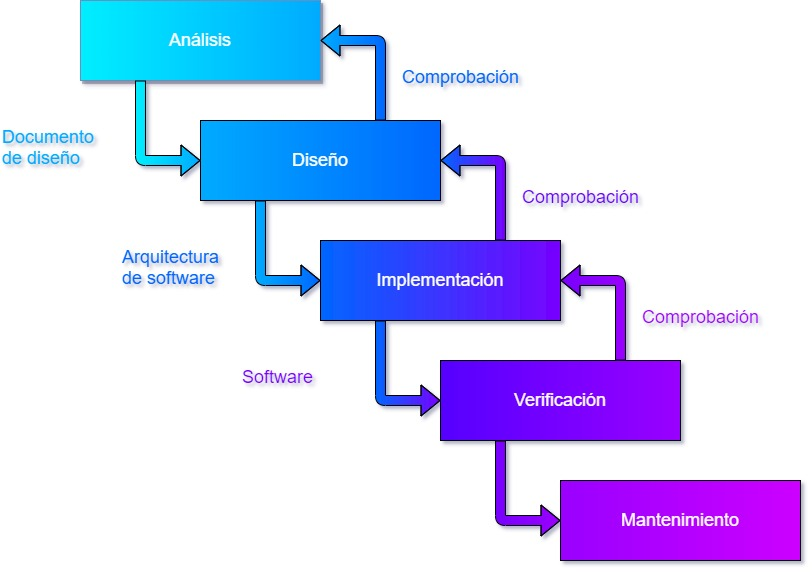
\includegraphics[width=5cm]{Figures/modelo_cascada.jpg}
        \caption{Modelo de desarrollo en cascada}
    \end{figure}

    \item \textbf{Desarrollo en espiral}: Este modelo, presentado por \textbf{Barry Boehm}, permite analizar con mayor profundidad 
    las etapas comprendidas en el desarrollo de un producto software. Las actividades de este modelo se conforman en una espiral, 
    en la que cada bucle o iteración representa un conjunto de actividades. Las actividades no están fijadas a ninguna prioridad, 
    sino que las siguientes se eligen en función del análisis de riesgo, comenzando por el bucle interior.

    \begin{figure}[H]
        \centering
        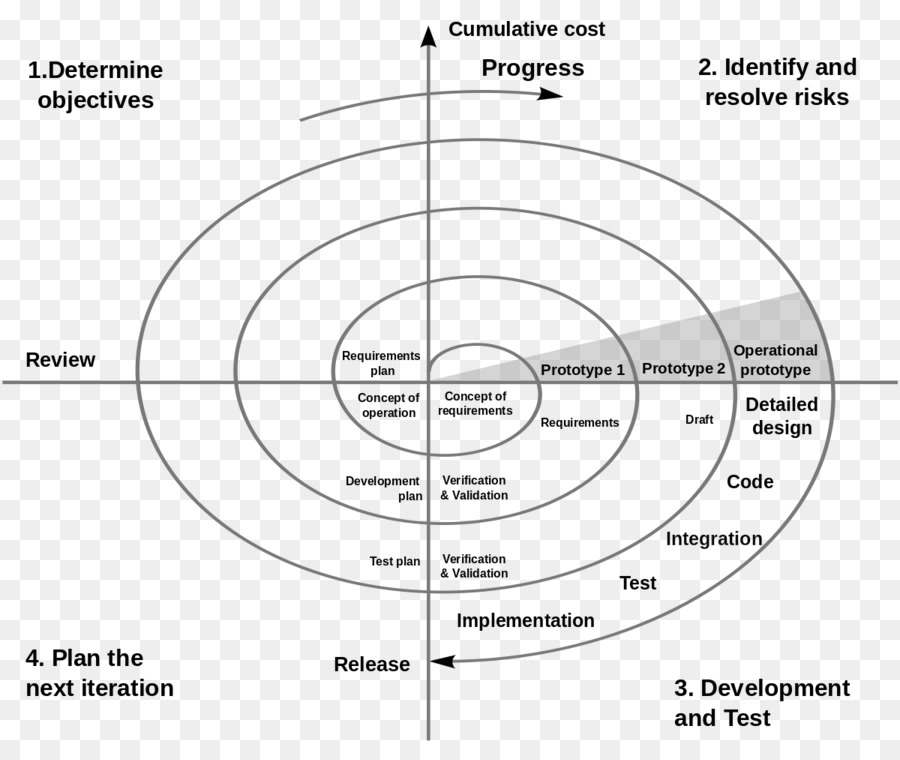
\includegraphics[width=5cm]{Figures/modelo_espiral.jpg}
        \caption{Modelo de desarrollo en espiral}
    \end{figure}

    \item \textbf{Desarrollo con prototipos}: \textit{El desarrollo de software basado en prototipos promueve la comunicación entre el cliente
    y el equipo de programadoroes, a la vez que logra una rápida integración de cambios y acorta el tiempo de desarrollo del proyecto.}
    (Ventura, Salinas, Álamos y Arreola, 2015). El paradigma de desarrollo basado en prototipos consiste en un proceso iterativo que tiene cinco 
    fases:
    % RAMÓN VENTURA ROQUE HERNÁNDEZ, JUAN MANUEL SALINAS ESCANDÓN, CALEB ALFREDO ÁLAMOS ACOSTA, ROBERTO ARREOLA RIVERA
    %Comparación empírica entre el proceso unificado y el desarrollo de software por prototipos. 
    \begin{enumerate}
        \item \textbf{\textit{Comunicación}}: Se indica un conjunto de objetivos que el software debe cumplir.
        \item \textbf{\textit{Plan rápido}}: Se propone una estrategia para llevar a cabo el desarrollo
        \item \textbf{\textit{Diseño rápido}}: Se realiza el diseño de una interfaz gráfica rápidamente.
        \item \textbf{\textit{Construcción}}: Se construye el prototipo del sistema software.
        \item \textbf{\textit{Entrega y retroalimentación}}: Se entrega el prototipo y el cliente realiza una 
        retroalimentación al equipo, que da inicio a una nueva iteración que incorpora los ajustes indicados en la 
        información dada por el cliente.
    \end{enumerate}
    
    \begin{figure}[H]
        \centering
        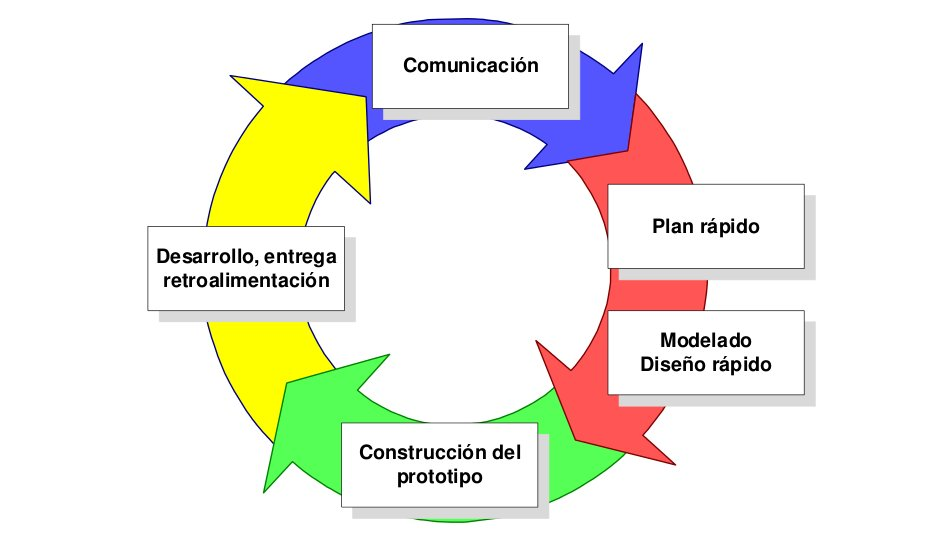
\includegraphics[width=5cm]{Figures/modelo_prototipos.jpeg}
        \caption{Modelo de desarrollo con prototipos}
    \end{figure}

    \item \textbf{Desarrollo incremental}:Consiste en un modelo iterativo que cuenta con una serie de fases de desarrollo
    (Análisis, Diseño, Implementación, Pruebas) que se repiten en orden de manera que cada vez que se finaliza una iteración, 
    el producto está mas refinado, siendo el objetivo llegar al producto final.

    \begin{figure}[H]
        \centering
        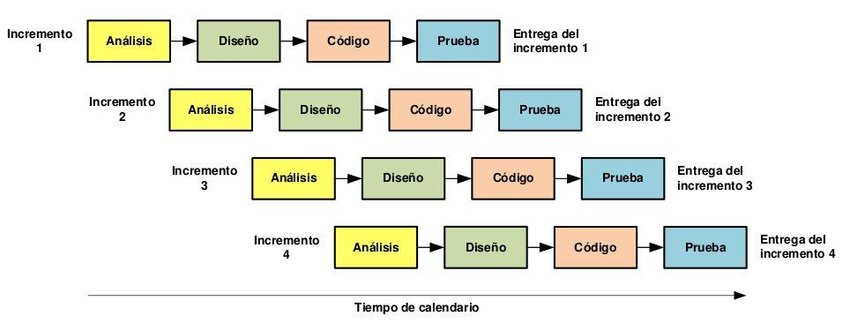
\includegraphics[width=8cm]{Figures/modelo_incremental.png}
        \caption{Modelo de desarrollo incremental}
    \end{figure}
\end{itemize}

\subsection{Metodologías Ágiles}
En febrero de 2001 nace el término \textbf{ágil} aplicado al desarrollo de software, tras una reunión celebrada en 
\textit{Utah (EEUU)}. El objetivo de la misma fue esbozar valores y principios que deberían permitir desarrollar 
software de manera rápida, dando respuesta a los cambios surgidos durante el desarrollo del proyecto. Se pretende 
con esto ofrecer alternativas a los procesos de desarrollo software tradicionales, rígidos y dirigidos por la documentación 
que se generaba en cada una de las etapas del proceso.\medskip

El punto de partida para ello fue el \textbf{Manifiesto Ágil}: %agilemanifesto.org
documento que resume la filosofía ágil, en el cual se valoran los siguientes elementos:
\begin{itemize}
    \item \textbf{El individuo y las interacciones del equipo de desarrollo sobre el proceso y las herramientas}:
    Las personas que forman parte del proyecto son el principal factor de éxito de un proyecto, de manera que el entorno
    influye menos que la bondad del equipo que realiza el desarrollo. Es preferible que el entorno se adapte al equipo.

    \item \textbf{Desarrollo de software útil es mejor que conseguir una buena documentación}:
    La regla a seguir es \textit{producir sólo documentos que sean necesarios inmediatamente para tomar una 
    decisión importante}.

    \item \textbf{La colaboración del cliente sobre la negociación de un contrato}: Se propone una interacción 
    constante entre cliente y desarrolladores, de manera que esta colaboración permita marcar el ritmo del 
    proyecto y asegure el éxito del mismo.

    \item \textbf{Respuesta rápida a los cambios es mejor que seguir un plan de forma estricta}:
    La habilidad de responder a los cambios determina el éxito o fracaso del proyecto, de manera que lo
    más importante de la planificación es su flexibilidad.
\end{itemize} 

Los principios del \textit{Manifiesto Ágil} se basan en estos valores, que a su vez hacen de fundamentos de 
todas las metodologías ágiles, orientando el desarrollo a la rápida obtención de un producto funcional 
aunque no tenga todas sus funciones implementadas. \medskip

Del modelo de desarrollo ágil se pueden encontrar diversas metodologías, como \textbf{eXtreme Programming} (Stephens \& Rosenberg, 2003),
\textbf{Scrum} (Sutherland \& Schwaber, 2010) o \textbf{Crystal Clear} (Cockburn, 2004). 
Para este proyecto se ha tomado la decisión de seguir la metodología \textit{\textbf{Scrum}} ya que debido a la naturaleza y complejidad del mismo, 
es posible que sea necesario realizar cambios en el planteamiento del proyecto durante el proceso de desarrollo. \medskip

\subsection{SCRUM}
\begin{figure}[H]
    \centering
    
\includegraphics[width=5cm]{Images/Logo_Scrum.jpeg}
    \caption{Logo de \textit{Scrum}}
\end{figure}

\subsubsection{Introducción}
\textit{SCRUM} es una de las metodologías de desarrollo ágil más reconocidas mundialmente. Su concepción resulta de unos 
análisis realizados por \textbf{Ikujiro} \textbf{Nonaka} e \textbf{Hirotaka} \textbf{Takeuchi} en los años 80, resaltando el trabajo en equipo para el 
desarrollo de productos y la autonomía que estos deben tener (Takeuchi \& Nonaka, 1986). Su diseño se debe a que 
en los años 90, \textbf{Jeff} \textbf{Sutherland} y \textbf{Ken} \textbf{Schwaber} formalizaron un marco de trabajo y unas reglas aplicadas 
particularmente al desarrollo de software de productos complejos (Schwaber \& Sutherland, 2012). \medskip % Por qué implementar SCRUM

\subsubsection{Características}
A continuación se muestra una serie de características que deben tener todos los procesos que se introducen al marco 
de la metodología \textit{Scrum}:
\begin{itemize}
    \item El desarrollo incremental de los requisitos en bloques temporales cortos y fijos.
    \item Se da prioridad los requisitos más valorados por el cliente.
    \item El equipo se sincroniza diariamente y se realizan las adaptaciones necesarias.
    \item Tras cada iteración se muestra el resultado real al cliente, para que tome las decisiones 
    necesarias en relación al resultado observado.
    \item Se le da al equipo la autoridad necesaria para poder cumplir los requisitos.
    \item Fijar tiempos máximos para lograr objetivos.
    \item Equipos de trabajo pequeños (de 5 a 9 personas).
\end{itemize}

\subsubsection{Ciclo de desarrollo}
Para entender el ciclo de desarrollo de \textit{Scrum} es necesario conocer las fases que lo definen:
\begin{enumerate}
    
    \item \textbf{Planificación}: Reunión de los involucrados en la que se definen los requisitos prioritarios para 
    la iteración actual y se elabora una lista de tareas necesarias para lograr los requisitos previamente seleccionados.

    \item \textbf{Scrum diario}: Evento del equipo de desarrollo de quince minutos, que se realiza diariamente durante la
    ejecución de la iteración para explicar lo que se ha alcanzado desde la última reunión, lo que se hará antes de la 
    siguiente y los obstáculos que se han presentado. 

    \item \textbf{Revisión}: El equipo presenta al cliente los requisitos completados en la iteración. En función de los 
    resultados mostrados y de los cambios habidos en el contexto del proyecto, el cliente realiza las adaptaciones 
    necesarias de manera objetiva, replanificando el proyecto.

    \item \textbf{Retrospectiva}: El equipo analiza cómo ha sido su manera de trabajar y qué problemas podrían impedirle 
    progresar adecuadamente, mejorando de manera continua su productividad.
\end{enumerate}

\begin{figure}[H]
    \centering
    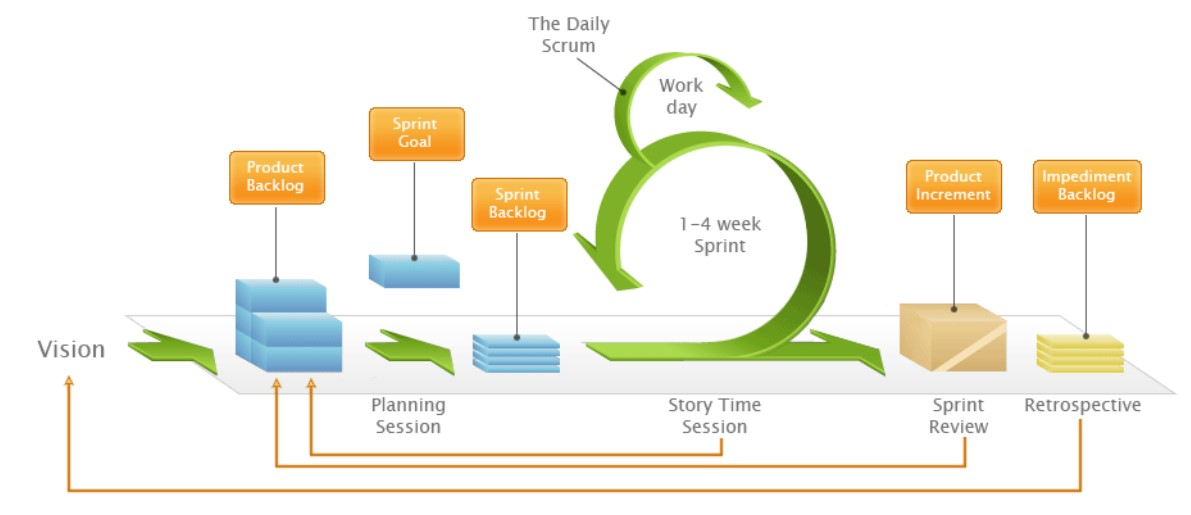
\includegraphics[width=14cm]{Images/Ciclo_Scrum.jpg}
    \caption{Ciclo de desarrollo de \textit{Scrum}}
\end{figure}

\subsubsection{Roles}
Los roles presentes en \textit{Scrum} son los siguientes:
\begin{itemize}
    \item \textbf{Product Owner}: Tiene la responsabilidad de decidir qué trabajo necesita hacerse, y maximizar el valor 
    del proyecto o producto que se esté llevando a cabo. Para ello debe tener las siguientes cualidades:
    \begin{enumerate}
        \item \textit{Saber gestionar prioridades}: Es responsable de gestionar los presupuestos, de contratar al equipo de 
        desarrollo y de explicar cuál es el valor que produce el producto en el que está invirtiendo.
        \item \textit{Toma de decisiones}: Debe ser capaz de tomar decisiones por su cuenta.
        \item \textit{Coordinador}: Tiene que poder medir el valor generado y utilizar la flexibilidad de entregar cada 
        \textit{sprint} para incrementar ese valor.
    \end{enumerate}
    
    \item \textbf{Scrum Master}: Persona que ayuda al equipo y a la organización a optimizar el uso de la 
    metodología. Traslada la visión del proyecto al equipo, y elimina los obstáculos que impiden que el equipo alcance el 
    objetivo del \textit{sprint}.

    \item \textbf{Development Team}: Grupo de profesionales con los conocimientos técnicos necesarios y que desarrollan el proyecto de manera
    conjunta llevando a cabo los requisitos a los que se comprometen al inicio de cada \textit{sprint}.
\end{itemize}

\begin{figure}[H]
    \centering
    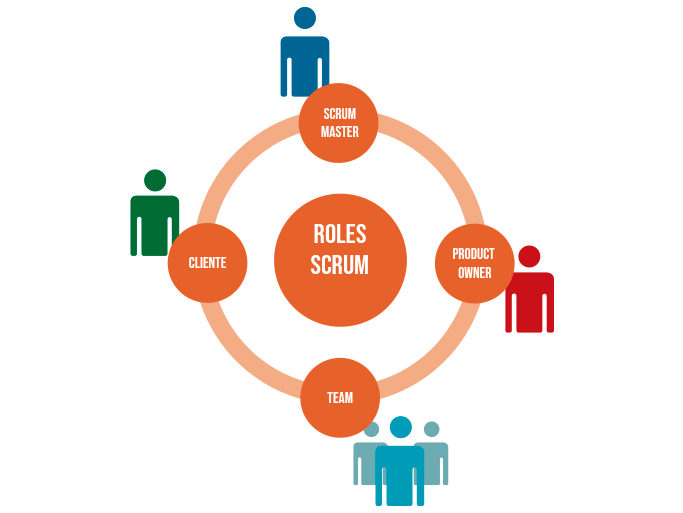
\includegraphics[width=10cm]{Images/roles.png}
    \caption{Roles en \textit{Scrum}}
\end{figure}